\documentclass[10pt]{article}
\usepackage[utf8]{inputenc}
\usepackage{graphicx}
\usepackage{xcolor}
\usepackage{calc}
\usepackage[shortlabels]{enumitem}

\newcounter{tablemajor}
\renewcommand\thetable{\arabic{tablemajor}}
\newcommand*\settablecounter[1]{%
        \setcounter{tablemajor}{#1}%
}

\newcounter{figuremajor}
\renewcommand\thefigure{\arabic{figuremajor}}
\newcommand*\setfigurecounter[1]{%
        \setcounter{figuremajor}{#1}%
}

\setlength{\parindent}{0pt}

\title{On Scalable DCEL Overlay Operations\\{\large Response to the Reviewers}}
\author{}

\begin{document}
\maketitle
Thank you for giving us the opportunity to submit a revised draft of our manuscript for publication.  We appreciate the time and effort that you and the reviewers have dedicated to providing your valuable feedback on our paper.  We have been able to incorporate changes to reflect most of the suggestions provided by the reviewers. Those changes are highlighted within the manuscript.  Please see below for a point-by-point response to the reviewers’ comments and concerns. The authors welcome further constructive comments if any.

\section*{General Comments to the Authors:}
\subsection*{Comment 1}
\textit{
The paper implements overlay operators using the Apache Spark framework, however, a map-reduce description of input partitioning, load balancing, local operations, and optimizations, with Spark-specific transformations and actions for the implementation, is not presented in any level of detail.
} \\

\textbf{Author Response:}\\

Thank you about this remark.  We tried to avoid technical references to a specific platform but we find interesting your comment and add some details about the Apache Spark specific transformations and actions at the end of section 7.  Please see below the lines we add about the topic.\\

\textbf{\textcolor{blue}{
``The scalable approach was implemented over the Apache Spark framework.  From a Map-Reduce point of view the stages described in Section 4 were implemented using several transformations and actions supported by Spark.  For example, the partitioning and load balancing described in Section 4.1 and 6.3 was implemented using a Quadtree, where its leaves were used to map and balance the number of edges that have to be sent to the worker nodes.  Mostly, map operations were used to transform and locate the edges in the corresponding leaf to exploit proximity among them at the same time that it divided the amount of work in an evenly manner.
Similarly, the edges at each partition were processed using chains of transformations at local level (see Section 4) followed for actions such as reducers to post-process incomplete faces which could span over multiples partitions and have to be combined or re-distributed to obtain the final answer.  In addition, the reduce procedures were further explored through some optimizations as it was described in Section 5.''
}}

\subsection*{Comment 2}
\textit{
The experimental section includes new content, different from the published conference papers, however, the impact of shuffle, i.e., communication cost warrants more discussion.
} \\

\textbf{Author Response:}\\

Thanks about your comment.  We found valuable to include the following paragraph to discuss in particular the implact of the Kdtree partitioning and overlay procedures over re-distribution of data and the involved communication cost it could generate. It was added in Section 7.5.\\

\textbf{\textcolor{blue}{
``Note that although the Kdtree creation takes more time, both the partitioning and overlay operations present better performance over the Quadtree partition strategy.  As was said before, the smaller number of leaves, with and without edges, has also a direct impact on the communication cost as the shuffle operations have to deal with considerably less number of partitions.''
}}

\section*{Specific Comments to the Authors:}
\subsection*{Comment 1}
\textit{Abstract\\
Please clarify if the approach is only applicable to planar/projected data. In the case of data with only a Geographic Coordinate System, why would the current approach not be applicable?} \\

\textbf{Author Response:}\\

\textbf{\textcolor{blue}{
``The Doubly Connected Edge List (DCEL) is an edge-list structure widely utilized in spatial applications for mainly planar topological and geometric computations although is also applicable to diverse kinds of data (i.e. 3D models, geographic data).''
}}

\subsection*{Comment 2}
\textit{
Section 4 \\
Could you provide a reference to the sequential base implementation used to test DCEL generation on the Main US dataset?
} \\


\textbf{Author Response:}\\

\textbf{\textcolor{blue}{
``In order to test the scalable approach, a sequential algorithm for DCEL creation was created following the pseudo-code presented in \cite{berg_computational_2008}.''
}}

\subsection*{Comment 3}
\textit{
Section 4.1\\
It is not clear what the authors mean by "(in the number of edges)".
} \\


\textbf{Author Response:}\\

``One could use a simple grid to divide the spatial area, but our early experiments showed that such an approach would result in unbalanced cells
\textbf{\textcolor{blue}{
where some cells will have significantly more edges than others which will affect the overall performance.''
}}

\subsection*{Comment 4}
\textit{
Section 4.2\\
Can the authors provide more insight on the average and worst cases on how long it takes for Algorithm 1 to converge on a miss, i.e., when all three cells are orphans?
} \\


\textbf{Author Response:}\\

\textbf{\textcolor{blue}{
``To find the worst-case performance of the search algorithm, we note that given an orphan cell, the algorithm performs three-point quadtree queries to find the leaves of the siblings that contain the centroid.
It then picks one of the found leaves as above and asks three-point queries for a new centroid to the siblings of that leaf etc. As a result, the algorithm explores the quadtree always going deeper. The worst case would be the longest path of a quadtree which can be $O(N)$. In the average case, i.e., when the quadtree is balanced, it is logarithmic.''
}}

\subsection*{Comment 5}
\textit{
Section 5\\
"boundaries of faces that expand different cells". expand vs span - is a cell expanding vs is a face extended/spanning over multiple cells? Currently, it makes the reader believe the cell is being expanded during a quadtree build, which in reality isn't the case. Please clarify the text and Section 5.1 title.
} \\

\textbf{Author Response:}\\

\textbf{\textcolor{blue}{
``Optimizations for faces spanning over multiple cells''
}}

\subsection*{Comment 6}
\textit{
Section 5.1\\
``the user can specify a level in the quadtree structure (measured as the depth from the root) that can be used to combine cells together". In reality, a user has no prior insight for how the quadtree will look as it will depend on the data. Even worse, the user cannot predict the impact of selecting a level for reduction. The effect of data partitioning, and shuffle time has an impact on achievable parallelism. Section 5 and Section 7 do not explain these effects when considered together in the application.
} \\

\textbf{Author Response:}\\

\textbf{\textcolor{blue}{
``Although a prior value for the level is difficult to set, it can be based on the size of the input.  In addition,  Section 7.1 shows recommendations for possible values or alternative solutions.''
}}

\subsection*{Comment 7}
\textit{
Section 5.1\\
Overall, this section is difficult to follow without better presenting operations from a map-reduce standpoint. At each stage, what happens at the executors versus what happens at the driver? When do the jobs wait to synchronize or communicate? From a distributed computing standpoint, this information is not available to a reader.
} \\


\textbf{Author Response:}\\

$\cdots$
\textbf{\textcolor{blue}{``From a distributed point of view this is a typical map-reduce operation where in the map phase, each worker node reports faces that are completely contained in its boundary or segments of faces that could concatenate with other faces segments reported by other worker nodes.
Face segments are sent to a master node at a communication cost because it has to wait for all nodes to report possible segments.  Then, the master node groups segments by face ID, and sorts and concatenates the parts to form closed faces in the reduce phase.''}}
$\cdots$

$\cdots$
\textbf{\textcolor{blue}{``From a map-reduce standpoint, this alternative works similarly to the previous but it introduces additional reduce operations at the intermediate level.  However, note that this introduces new synchronization points since each new reducer has to wait for their workers to report possible face segments before processing them and reporting new faces or sent to the driver segments that were not completed at that level.''}}
$\cdots$

$\cdots$
\textbf{\textcolor{blue}{``From a distributed computing standpoint, this alternative adds a shuffle stage at the beginning but it avoids any reduce operation.  The shuffle places all the segments with the same ID in the same worker, so they can be processed and reported directly.''}}
$\cdots$

\subsection*{Comment 8}
\textit{
Section 5.2\\
``In the current approach" - did you mean in the naive approach?
} \\

\textbf{Author Response:}\\
\textbf{\textcolor{blue}{
``In our initial implementation}},
the input sets of half-edges within a cell are combined into one dataset, first ordered by the x-origin of each half-edge.''

\subsection*{Comment 9}
\textit{
Section 6.4\\
The operations described in this section would be easier to follow with an illustration using the running example in the paper
} \\

\textbf{Author Response:}\\
$\cdots$
\textbf{\textcolor{blue}{
``Figure~\ref{fig:dangleoverlay:input} shows the spatial partitioning of the two input layers $A$ and $B$. Layer $A$ has two input polygons: $A_0$ and $A_1$. Layer $B$ has three dangle edges $B_0$, $B_1$ and $B_2$.''
}}
$\cdots$

\setfigurecounter{14}
\begin{figure}[h!]
	\centering
	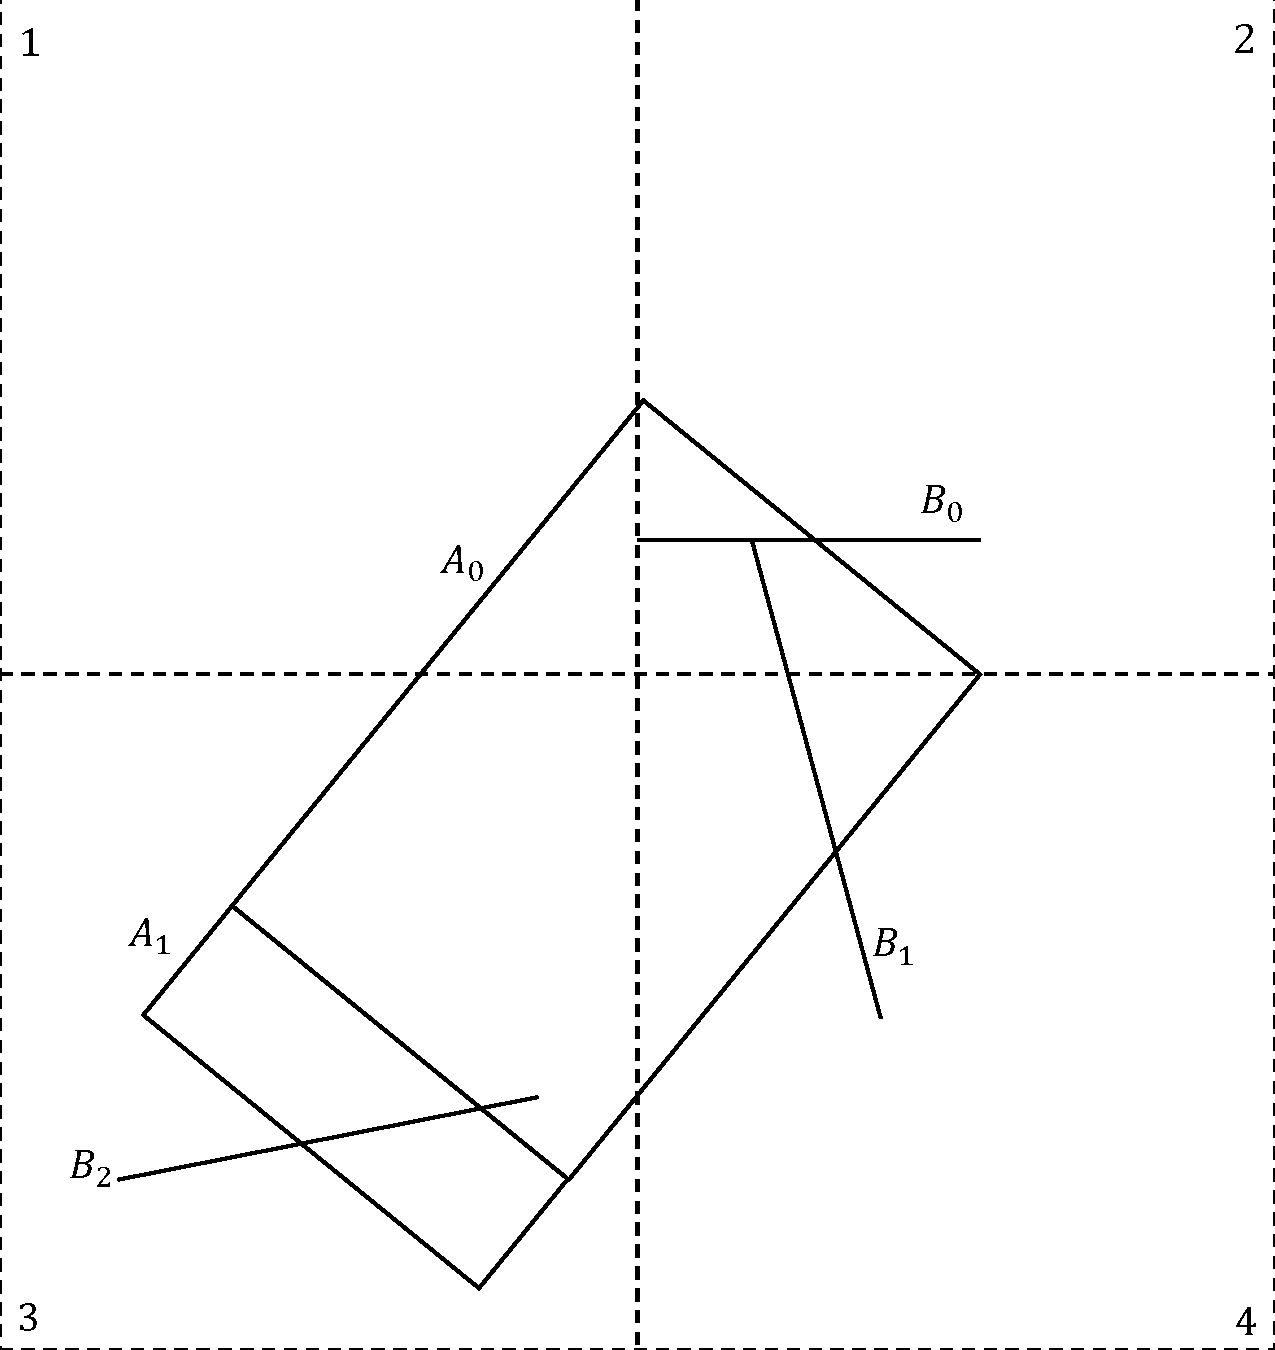
\includegraphics[width=0.5\linewidth ]{figures/DangleOverlay1.pdf}
	\caption[caption]{Spatial Partitioning of input layers A and B}
	\label{fig:dangleoverlay:input}
\end{figure}

$\cdots$
\textbf{\textcolor{blue}{
``In Figure~\ref{fig:dangleoverlay:inter}, Polygon $A_0$ is re-partitioned with edges it intersect with, namely $B_0, B_1$, and $B_2$.''
}}
$\cdots$

\setfigurecounter{15}
\begin{figure}[h!]
	\centering
	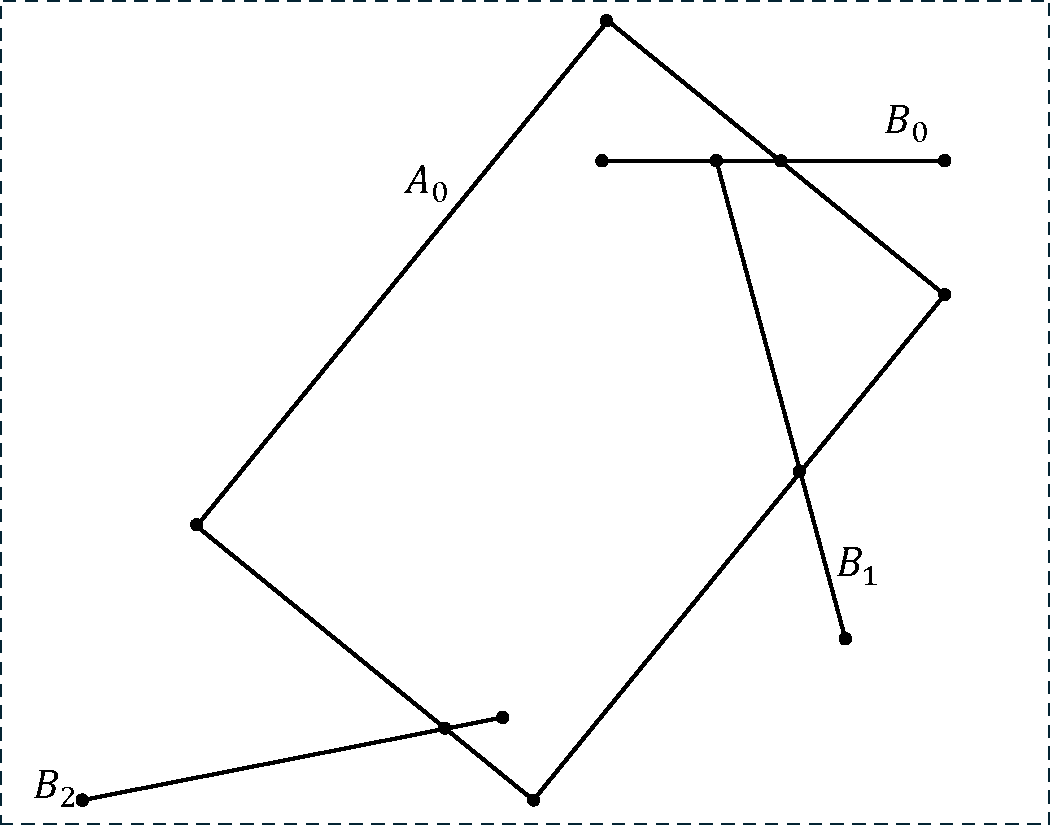
\includegraphics[width=0.55\linewidth ]{figures/DangleOverlay2.pdf}
	\caption[caption]{Re-Partitioning of Polygon $A_0$ with Edges it intersects with}
	\label{fig:dangleoverlay:inter}
\end{figure}

$\cdots$
\textbf{\textcolor{blue}{
``Figure~\ref{fig:dangleoverlay:result}, shows the result of polygonization of edges from Polygon $A_0$ and $B_0$, $B_1$, and $B_2$, resulting two polygons $A_01$ and $A_02$.''
}}
$\cdots$

\setfigurecounter{16}
\begin{figure}[h!]
	\centering
	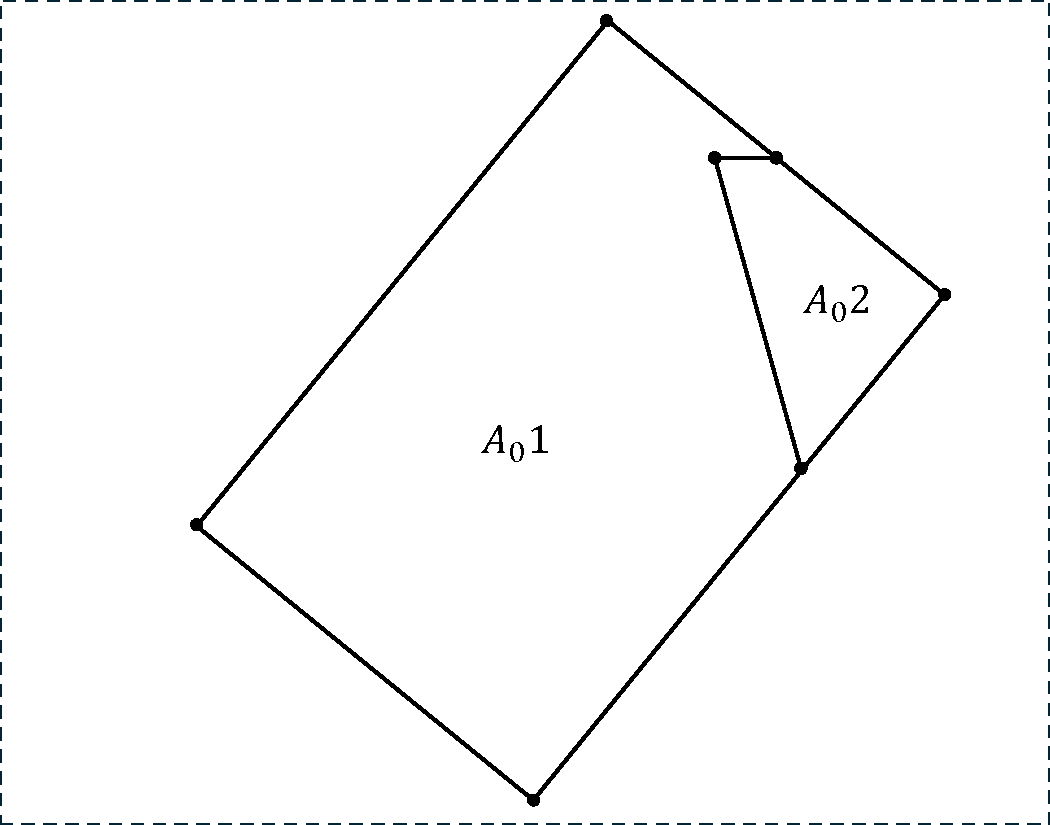
\includegraphics[width=0.55\linewidth ]{figures/DangleOverlay3.pdf}
	\caption[caption]{The result of polygonization of $A_0$ with $B_0, B_1, B_2$}
	\label{fig:dangleoverlay:result}
\end{figure}

\subsection*{Comment 10}
\textit{
Section 7.1\\
The section will benefit from stats such as the number of holes, empty cells, and orphan cells generated.
} \\

\textbf{Author Response:}\\
\textbf{\textcolor{blue}{
``Table \ref{tab:orphans} shows the number of cells, original holes, and orphans cells and holes generated after partitioning using the optimal values.''
}}

\settablecounter{6}
\begin{table}[h!]
    \centering
    \caption{Orphan cells and orphan holes description}
    \label{tab:orphans}
    \begin{tabular}{c c c c}
        \hline
                &          &          & Number       \\
                & Number   & Number   & of orphans   \\
        Dataset & of cells & of holes & (cell/holes) \\
        \hline
        GADM  & 21970      & 1999     & 4310 \\
        MainUS& 12343      & 850      & 1069 \\
        CCT   & 7124       & 40       & 215  \\
        \hline
    \end{tabular}
\end{table}

\subsection*{Comment 11}
\textit{
Section 7.1\\
``for each state experiment, we tried different numbers of leaf cells for the quadtree and presented the one with the best performance.". Please state the quadtree parameters to help the reader make an informed selection decision.
} \\

\textbf{Author Response:}\\

\textbf{\textcolor{blue}{
``Note that for each state experiment, we tried different numbers of cells for the quadtree and presented the one with the best performance. For this, we sample 1\% of the edges of each state and evaluate the best number of cells varying from 200 cells to 2000.  Most of the states get the optimal value around 3000 cells.''
}}

\subsection*{Comment 12}
\textit{
Section 7.2\\
The experiments demonstrate a speedup of the order of milliseconds. The contribution of the filtered-sweep algorithm in the final runtime on large datasets is not available.
} \\

\textbf{Author Response:}\\

\textbf{\textcolor{blue}{
``It is expected that in datasets with significant differences in the distribution of edges between layers, the improvement at the cell level can sum up enough to impact positively the overall performance.''
}}

\subsection*{Comment 13}
\textit{
Section 7.3\\
The parenthesized statements can be stated directly if they are relevant to the experiment.
} \\

\textbf{Author Response:}\\
It is fixed along section 7.2 and in overall in all the manuscript.

\subsection*{Comment 14}
\textit{
Section 7.3\\
It is not clear what impact data shuffle has on the runtime, if any. Specifically, does the size of data partitions have an impact on the runtime? What is the min/max/average size of a cell?
} \\

\textbf{Author Response:}\\

\textbf{\textcolor{blue}{
``In addition, table \ref{tab:cell_stats} shows some statistics for the cells at the optimal values.  It can be seen that in the larger datasets, an average cell size of $\approx$3000 edges will give the best results. That cell size will imply a relatively small amount of data to be transmitted which will have a low impact on data shuffle and data processing.''
}}

\settablecounter{5}
\begin{table}[h!]
    \centering
    \caption{Cell size statistics.}
    \label{tab:cell_stats}
    \begin{tabular}{ccccccc}
        \hline
        Dataset & Min & 1st Qu. & Median & Mean & 3rd Qu. & Max   \\
        \hline
        GADM    & 0   & 0       & 2768   & 3141 & 5052    & 16978 \\
        MainUS  & 0   & 1538    & 2582   & 2853 & 3970    & 10944 \\
        CCT     & 0   & 122     & 324    & 390  & 546     & 1230  \\
        \hline
    \end{tabular}
\end{table}

\subsection*{Comment 15}
\textit{
Section 7.3\\
It is not clear how the quadtree splitting criteria is being controlled to create cells as a multiple of 1000 and not a multiple of 4.
} \\

\textbf{Author Response:}\\

\textbf{\textcolor{blue}{
``The quadtree settings allow for tuning its performance by providing the \textit{maximum capacity} of a cell as a parameter. The quadtree then continues its splits if it reaches this capacity. There is an inverse relationship between the capacity and the number of leaf cells in a quadtree.
A low capacity will lead to a large number of cells. On the other hand, large values for capacity imply a smaller number of divisions (noted that the final number of partitions would not necessarily be a multiple of 4, especially in skewed datasets).''
}}

\subsection*{Comment 16}
\textit{
Section 7.4\\
The speedup and scaling performance shown in Fig. 18 and Fig. 19 is impressive.
} \\

\textbf{Author Response:}\\
We agree but we have to clarify that in this case each node correspond one-to-to with a Spark executor.  Under this configuration each node/executor has 8 cores.

\subsection*{Comment 17}
\textit{
Section 7.5\\
``We can see that the kd-tree takes more time, particularly because of the sorting done at each split, to organize the data and localize the middle point." In the average case, this is indeed a true statement. It would be more interesting to the reader if this could be presented as a percentage of the total runtime.
} \\

\textbf{Author Response:}\\

\textbf{\textcolor{blue}{
``In average, Quadtree takes 23.13\% the time it takes for Kdtree to be created (21.55\% in MainUS and 24.72\% in GADM). However, the Kdtree creation is just the 5.86\% of the overall time during the total DCEL construction using a Kdtree (6.88\% in MainUS and 4.87\% in GADM).''
}}

\subsection*{Comment 18}
\textit{
Section 7.5\\
Fig. 23 - Is the x-axis correct? Were the experiments carried out with $21*10^6$ cells?
}\\

\textbf{Author Response:}\\
The issue was fixed in figure \ref{fig:k_overlay_us}.

\setfigurecounter{26}
\begin{figure}[h!]
    \centering
    {\tiny (a)}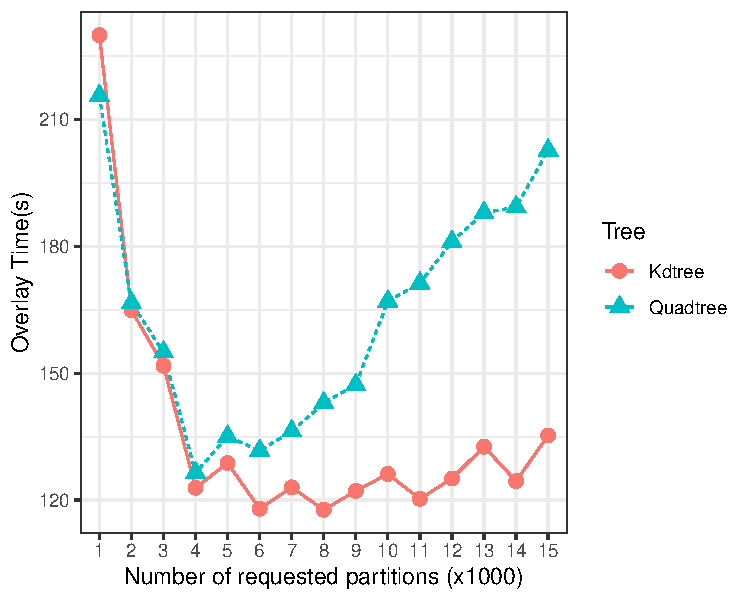
\includegraphics[width=0.45\linewidth]{figures/K_Overlay_US.pdf}
    {\tiny (b)}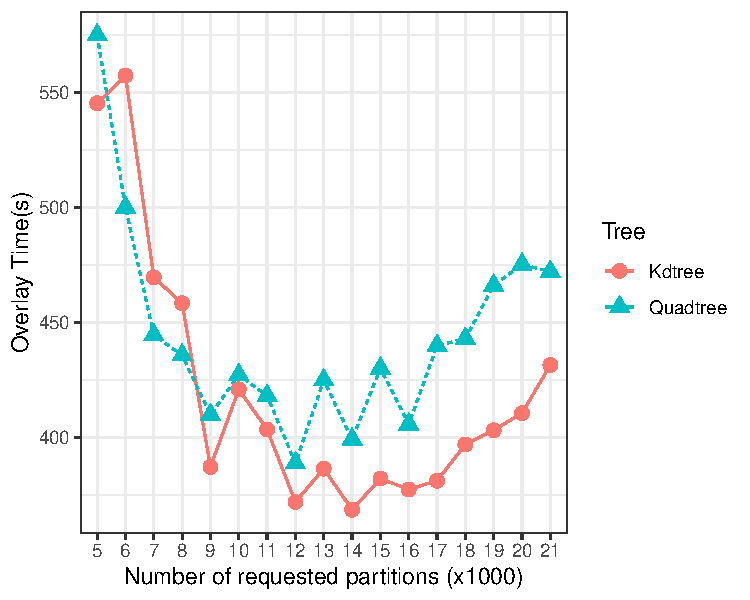
\includegraphics[width=0.45\linewidth]{figures/K_Overlay_GADM.pdf}
    \caption{Execution time for the overlay operation using a spatial data structure in the MainUS (a)and GADM (b) dataset.} \label{fig:k_overlay_us}
\end{figure}

\subsection*{Comment 19}
\textit{
Sections 7.6 and 7.7\\
``for datasets with close or similar cardinalities, the area of the dataset has a positive correlation with the build time". The experimental setup needs a better explanation. There are 12 nodes, of which executors are varied from 7 to 84.}

\begin{enumerate}[(a)]
\item \textit{
What is the count of executors per node?
} \\

\textbf{Author Response:}\\
Thanks for the remark.  We think we need to clarify the settings of the experiments in this section.  Below you can see what we added to explain the details of our configuration at the beginning of section  7.6.

\textcolor{blue}{
\textbf{
``We implemented our polygonization framework on Apache Sedona~\cite{sedona}.
The experiment is based on Java~8 implementation and uses a Spark~2.3 cluster of a dual-master node and 12~worker nodes. All nodes run Linux CentOS 8.2 (64bit).
Each master node is equipped with 128GB RAM, and each worker node is equipped with 64GB RAM.
To increase parallelism, We divide the 12 worker nodes of 64GB RAM into 84 worker executors each with 4GB RAM. Each executor is a separate JVM process with dedicated resources like memory and CPU cores. This gives us a total of 84 worker executors.
The distribution of executors across the nodes depends on how resource negotiator (YARN) allocates resources for Spark jobs, based on available cores and memory. Given that YARN typically tries to balance resources across the cluster, the executors are likely to be evenly distributed, though some variation may occur based on resource availability at runtime.
Assuming even distribution, each worker node is comprised of $\frac{84}{12} = 7$ worker executors.''
}} \\

\item \textit{
In the base case, why is there no one-to-one correspondence of nodes to executors (12:7)?
} \\

\textbf{Author Response:}\\

The total number of worker executors on the Spark cluster we used is 84, the choice of a base of 7 executors was to show the effect of adding the same amount of executors (7) at each step till we reach the maximum number of executors (84).

We add the below paragraphan in section 7.7 to clarify the situation.

\textcolor{blue}{\textbf{
``At each step in the figure, we add 7 more executors which is roughly equivalent to adding 1 node.''
}}

\item \textit{Possible typo in 10.2M $Mkm^2$}\\

\textbf{Author Response:}\\

Thanks, this typo was fixed in section 7.6.

\end{enumerate}

\subsection*{Comment 20}
\textit{
Section 7.8\\
The section will benefit from stats such as the number of dangles and cut edges generated/resolved.
} \\

\textbf{Author Response:}\\

We agree about this suggestion.  We add the following text and table at the beginning of section 7.8.\\

\textcolor{blue}{\textbf{
``Table~\ref{tab:dangles} shows the number of polygons for each state for the first layer of the overlay. It also shows the number of dangle and cut edges per state for the second layer of the overlay. Finally, it shows the number of resultant polygons per state.''
}}

\settablecounter{8}
\begin{table}[h!]
    \caption{Overlaying Polygons with Dangle and Cut Edges Dataset}
    \label{tab:dangles}
    \begin{tabular}{c c c c}
        \hline
        Dataset & Number Layer $A$ of Polygons & Number of Layer $B$ Edges & Result Polygons \\
        \hline
        TN & 1,272 & 3,380,780 & 41,761 \\
        GA & 1,633 & 4,647,171 & 49,125 \\
        NC & 1,272 & 7,212,604 & 22,413 \\
        TX & 4,399  & 8,682,950 & 98,635 \\
        VA & 1,554 & 8,977,361 & 38,941 \\
        CA & 7,038 & 9,103,610 & 96,916\\
        \hline
    \end{tabular}
\end{table}

\subsection*{Comment 21}
\textit{
References\\
Please maintain the capitalization style of names and approaches in the paper titles.
} \\

\textbf{Author Response:}\\

Thank you for your remark.  The reference files were cleaned and corrected about this concern.

% \subsection*{Comment }
% \textit{
%
% } \\
%
% \textbf{Author Response:}\\

\begin{thebibliography}{9}

\bibitem{berg_computational_2008}
Berg, M., Cheong, O., Kreveld, M., Overmars, M.: Computational Geometry: Algorithms and Applications. Springer, TU Eindhoven, P.O. Box 513 (2008)
\bibitem{sedona}
Yu, J., Zhang, Z., Sarwat, M.: Spatial Data Management in Apache Spark: the GeoSpark Perspective and Beyond. GeoInformatica (2018)

\end{thebibliography}

\end{document}
